\chapter{Scenario Series 0}
\label{ap:scenario_series_0}

This appendix presents simulation results from the 0 scenario series, which tests impact of distributed versus centralized assumptions regarding agent supply planning behaviour. 

\section{Summary}
Table \ref{tab:scenario_list} below lists the scenarios in series 0. 
% Control scenario s0\_control simulates the base bilevel scenario.
% Agent fibre consumption behaviour is coherent with the anticipation mechanism built into our bilevel model.
% We assume that the industrial network is composed hardwood and softwood lines, which are operated independently (although there is convergence of these lines at the pulp mill).
% We also assume that each line ceases to consume fibre when doing so is no longer profitable. 
% More precisely, line-wise profitability must be non-negative, which means that each line will consume null-value fibre indefinitely until some other limiting constraint is encountered (supply, capacity, demand, etc).

% In our test dataset, profitable hardwood fibre consumption is limited to approximately 20000 units per period, which corresponds roughly to one-third of (classic, single-level) initial hardwood AAC.   
% Limiting hardwood fibre consumption to 20000 units forces the model to harvest high-softwood-content stands to supply the profitable softwood line.
% High-softwood-content stands are relatively scarce, and single-period agent planning horizon induces high-grading of the wood supply (relative to AAC).
% The cumulative result of this behaviour pattern is a rather striking decline in harvest levels and profits during the first seven planning cycles. 
% After this initial period of decline, harvest levels and profits rise and fall in a highly variable pattern, but never return to initial levels.

% Comparison scenario s0\_centralized eliminates the line-wise profitability constraint.
% This is equivalent to assuming centralized planning of the entire network (i.e., the basic LogiLab setup).
In this scenario, the agent may elect to operate the hardwood line at a net loss (i.e., consume more than 20000 units of hardwood) if this provides access mixedwood stands containing sufficient proportions of profitable softwood.
Relaxing the requirement for line-wise profitability indirectly widens the (hardwood) bottleneck on softwood supply, which has a significant impact on agent fibre consumption behaviour when AAC largely exceeds agent fibre requirement (i.e., principal uses the classic wood supply model: single level even-flow volume maximization, no anticipation constraints).
Although scenario s0\_centralized simulates much higher sustained harvest and profit levels than our control scenario, it is also much too optimistic about internal integration of agent decision-making behaviour. 
Our control scenario (and our bilevel algorithm) presents a more accurate simulation of \emph{status quo} principal and agent behaviour.

Scenario s0\_centralized is nonetheless useful as a best-case scenario from the agent's perspective (i.e., estimates an upper bound on agent performance, given \emph{status quo} principal behaviour). 
In other words the difference between scenario s0\_centralized and s0\_control is an estimate of potential improvement in agent's profit if network wood supply decisions were fully integrated (as opposed to partially distributed).

\begin{table}
  \centering
  \begin{tabular}{lll}
    \hline
    Scenario ID & Figure Reference & Description \\
    \hline
    0\_control & \ref{fig:s0_control} & Control scenario. \\
    0\_centralized & \ref{fig:s0_centralized} & Relax line-wise profitability constraint. \\
    \hline
  \end{tabular}
  \caption{Description of scenarios in series 6-4.}
  \label{tab:scenario_list}
\end{table}

Hardwood AAC attribution level is kept constant at 100\% for all scenarios. 
Softwood attribution levels above 100\% of AAC have no impact on model output, as softwood consumption is indirectly limited by hardwood AAC.
Limited availability of pure softwood stands forces the agent to harvest mixed stands, which in quickly saturates the hardwood line in the network.

More interesting is that declining profit and AAC can be observed at, and well below, 100\% softwood AAC attribution level. 
In fact, softwood attribution must be limited to 60\% of AAC to stabilise harvest level and profit over all 30 rolling-horizon replanning cycles.

Note that neither one of these scenarios could easily be described as sustainable. Profit and harvest levels jump around rather dramatically throughout the planning horizon, and the large gap between planned and executed harvesting activities negatively impacts the credibility of principal's repeated assurances if wood supply sustainability. Subsequent scenario series will test impact of replacing principal's current single-level wood supply model with our bilevel wood supply model. 

\section{Results}

Figures \ref{fig:s0_control} and \ref{fig:s0_centralized} present
simulation results for two scenarios. % Table \ref{tab:scenarios}
% summarizes scenario parameters used in the experiment for each
% scenario.
Disposition of figures is identical for all scenarios. The
first subfigure (a) for each scenario shows the initial
(ie. iteration-0) AAC solution. The second subfigure (b) for each
scenario shows first period of AAC solution for all 30 planning
iterations. The third subfigure (c) for each scenario shows the
implemented harvest level for all 30 planning iterations. Scenarios
3.1 and 3.2 also show profit in this subfigure on a secondary
axis. The fourth subfigure (d) for each scenario shows the difference
between initial and re-planned AAC. The fifth subfigure (e) for each
scenario shows the difference between re-planned AAC and harvest.  The
sixth subfigure (f) for each scenario shows the difference between
initial AAC and harvest. Softwood volume is shown with white bars,
hardwood volume with black bars, and total volume with small
circles. Profit (where applicable) is shown with the $\times$
symbol. 


\begin{figure}[h]
  \centering
  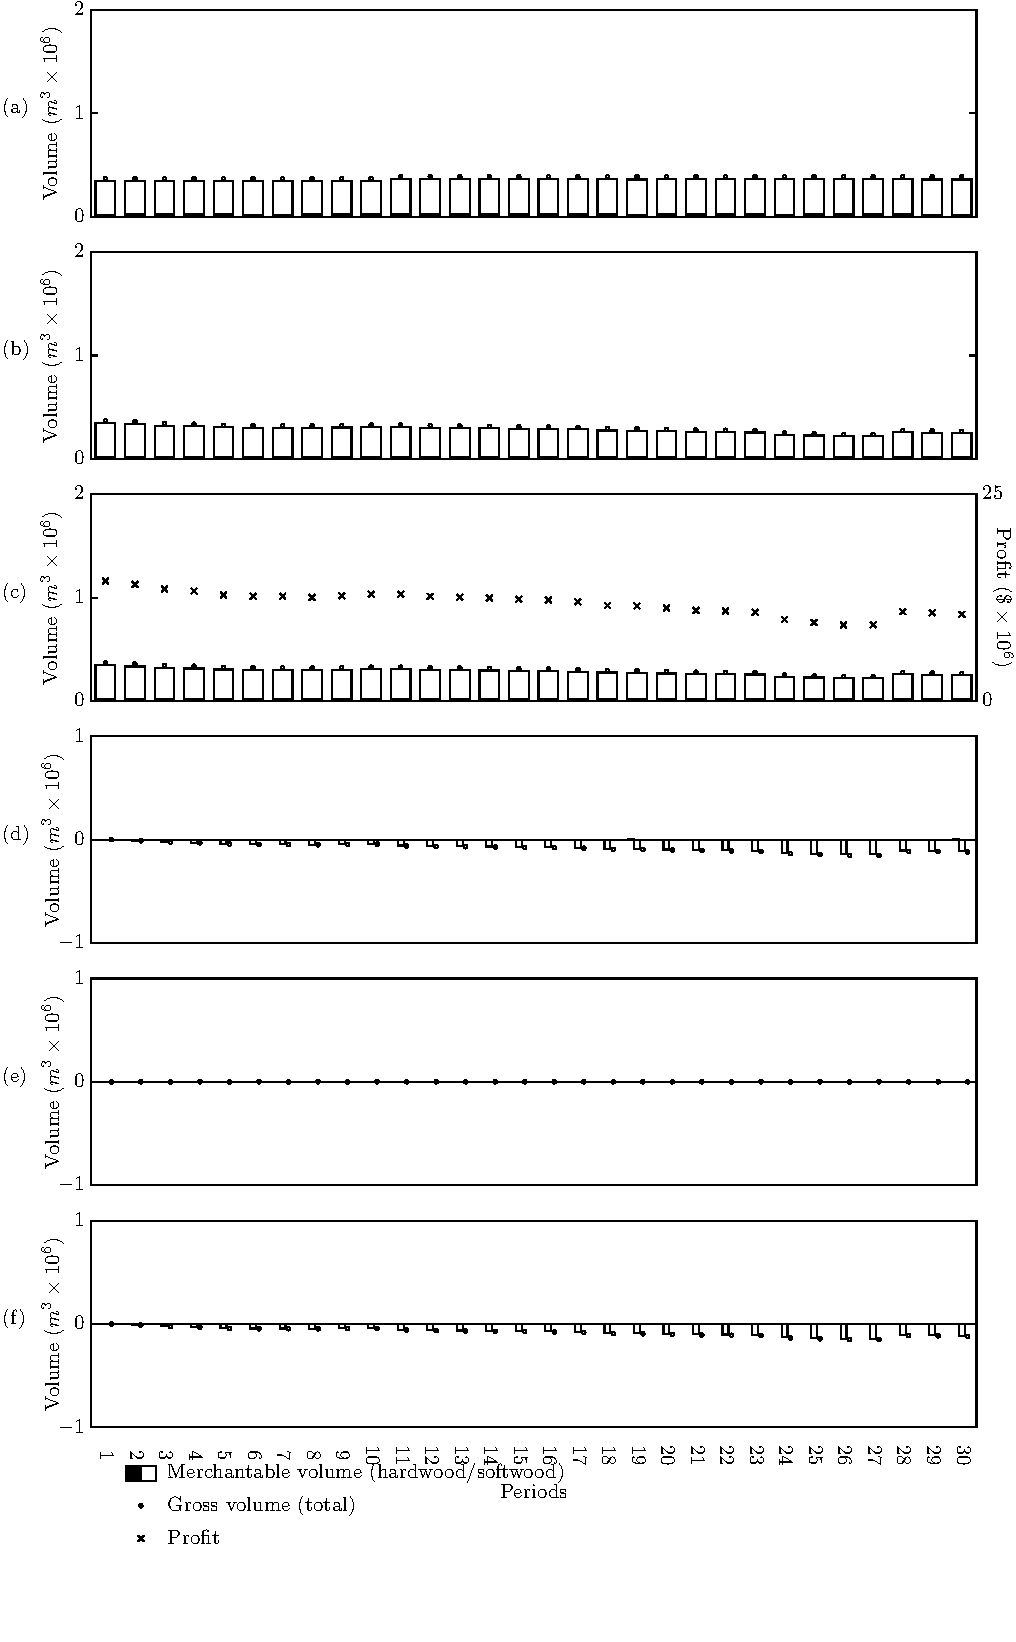
\includegraphics[width=10cm]{images/appendix/s6-1_p30a01}
  \caption{Reference sceanrio (i.e., base bilevel scenario)}
  \label{fig:s0_control}
\end{figure}

\begin{figure}[h]
  \centering
  \includegraphics[width=10cm]{images/appendix/s0_centralized}
  \caption{Scenario 0\_centralized (relax line-wise profitability constraint).}
  \label{fig:s0_centralized}
\end{figure}
